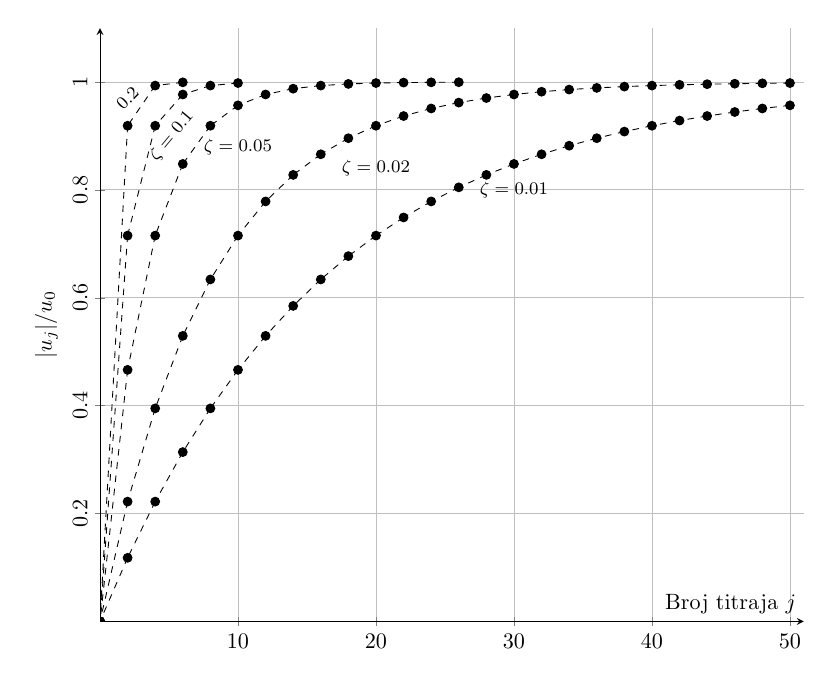
\begin{tikzpicture}[scale=0.8]
    \begin{axis} [
        height=11cm,
        axis lines=center,
        xlabel=Broj titraja $j$,
        ylabel={$|u_j|/u_0$},
        ylabel near ticks, ylabel style={anchor=south},
        xmin=0, xmax=51,
        ymin=0, ymax=1.1,
        xtick={0,10,20,30,40,50},
        ytick={0.2,0.4,0.6,0.8,1}, yticklabel style={rotate=90},
        grid=both,
    ]

        %zeta = 0.2
        \pgfplotsinvokeforeach{0, 2, 4, 6}
        {
            \filldraw( #1,{1 - exp(-2*pi*0.2*#1}) circle[radius=2pt, fill=black];
            \draw[dashed]( #1,{1 - exp(-2*pi*0.2*#1}) -- ( {#1-2}, {1-exp(-2*pi*0.2*(#1-2)});
        }

        %zeta = 0.1
        \pgfplotsinvokeforeach{0, 2, 4, ..., 10}
        {
            \filldraw( #1,{1 - exp(-2*pi*0.1*#1}) circle[radius=2pt, fill=black];
            \draw[dashed]( #1,{1 - exp(-2*pi*0.1*#1}) -- ( {#1-2}, {1-exp(-2*pi*0.1*(#1-2)});
        }

        %zeta = 0.05
        \pgfplotsinvokeforeach{0, 2, 4, ..., 26}
        {
            \filldraw( #1,{1 - exp(-2*pi*0.05*#1}) circle[radius=2pt, fill=black];
            \draw[dashed]( #1,{1 - exp(-2*pi*0.05*#1}) -- ( {#1-2}, {1-exp(-2*pi*0.05*(#1-2)});
        }

        %zeta = 0.02
        \pgfplotsinvokeforeach{0, 2, 4, ..., 50}
        {
            \filldraw( #1,{1 - exp(-2*pi*0.02*#1}) circle[radius=2pt, fill=black];
            \draw[dashed]( #1,{1 - exp(-2*pi*0.02*#1}) -- ( {#1-2}, {1-exp(-2*pi*0.02*(#1-2)});
        }

        %zeta = 0.01
        \pgfplotsinvokeforeach{0, 2, 4, ..., 50}
        {
            \filldraw( #1,{1 - exp(-2*pi*0.01*#1}) circle[radius=2pt, fill=black];
            \draw[dashed]( #1,{1 - exp(-2*pi*0.01*#1}) -- ( {#1-2}, {1-exp(-2*pi*0.01*(#1-2)});
        }

        %oznake
        \node at (30,0.80) {\footnotesize{$\zeta=0.01$}};
        \node at (20,0.84) {\footnotesize{$\zeta=0.02$}};
        \node at (10,0.88) {\footnotesize{$\zeta=0.05$}};
        \node[rotate=50] at (5.2, 0.9) {\footnotesize{$\zeta=0.1$}};
        \node[rotate=45] at (2, 0.97) {\footnotesize{$0.2$}};

        %ocitanja
%        \draw[thin] (0,0.95) -- (50,0.95);
%        %za 0.01
%        \draw[thin] (48,0) -- (48,0.95);
%        %za 0.02
%        \draw[thin] (24,0) -- (24,0.95);
%        %za 0.05
%        \draw[thin] (10,0) -- (10,0.95);
%        %za 0.1
%        \draw[thin] (5,0) -- (5,0.95);
%        %za 0.2
%        \draw[thin] (3,0) -- (3,0.95);
    \end{axis}
\end{tikzpicture}
